%  CONFIGURE NEW SINGLE-PAGE FORMAT 

\onecolumn % go back to one column
\fancyhead{} % make sure we get no headers
\renewcommand{\floatpagefraction}{0.1}
\lfoot[\bSupInf]{\dAuthor}
\rfoot[\dAuthor]{\cSupInf}
\newpage

\captionsetup*{format=largeformat} % make figure legend slightly larger than in the paper
\setcounter{figure}{0} % reset figure counter for the Supplementary Videos
%\setcounter{page}{1} % reset page count
\makeatletter
\renewcommand{\thefigure}{S\@arabic\c@figure} % videos numbered Movie S1, S2, ...
\makeatother
\renewcommand{\figurename}{Movie}

%  MAIN TEXT
\newpage
\section*{Supplementary Videos}

% Movie S1: transport_paper Working_notebooks/manuscript_figures/movie_s1.py (feat/flow-regime) -> manuscript/figures/movie_S1.mp4,
% copied to suppvideos/movie_S1.mp4 (H.264, 7.5 MB); the still is its first frame. Caption from the Typst supplement ("Movie").
\begin{SCfigure*}[50][!ht]
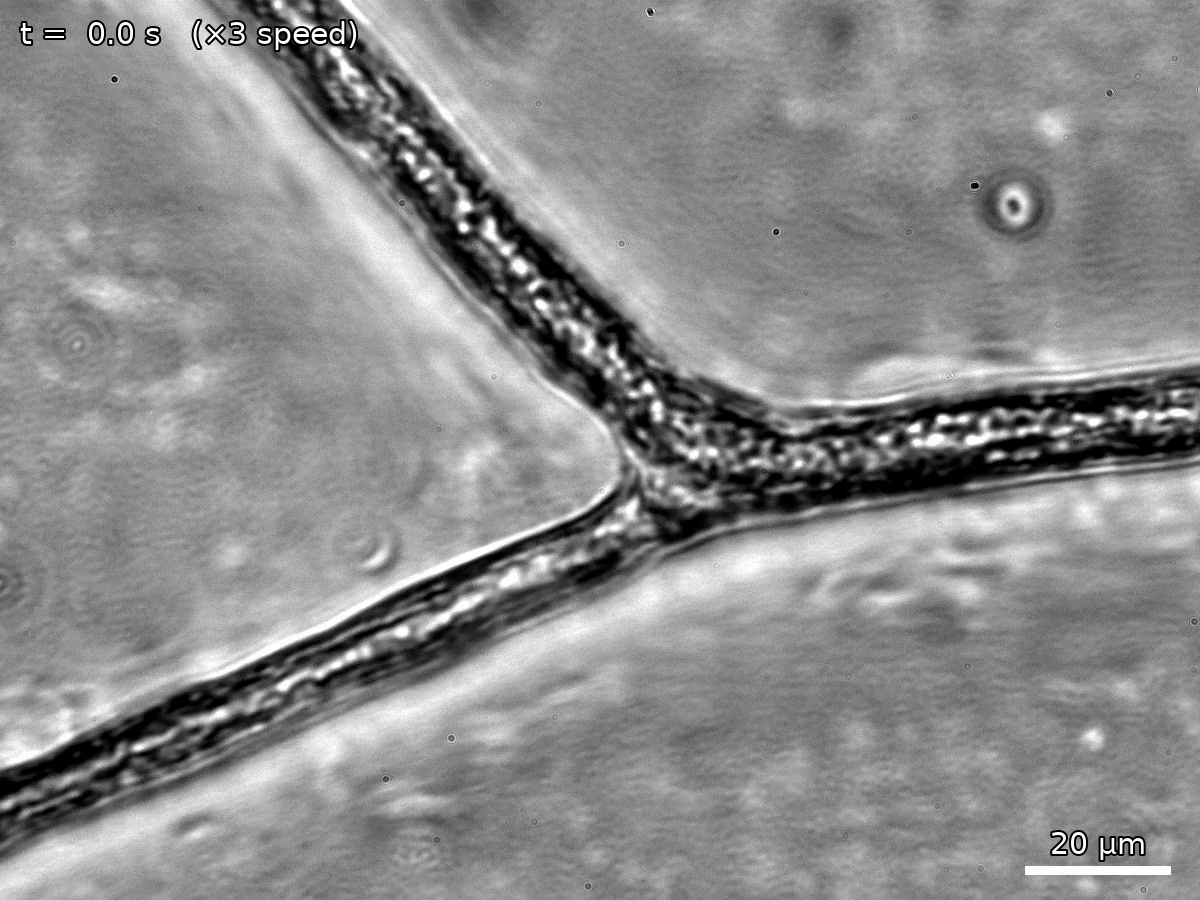
\includegraphics[width=0.5\linewidth]{suppvideos/movie_S1_still.png}
\caption{\textbf{Particles move both ways in the same hyphae.}\\
The flow video of Fig.~\ref{fig:hyphal_profiling}C: a junction on trail Middle of LPD2412A025 at day 12 (session t50), bright-field, 50$\times$ objective, 0.138~$\mu$m per pixel, recorded at 20 frames per second for 10~s.
Two frames averaged and played at 3$\times$ speed.\\
Time in seconds of recording. Scale bar, 20~$\mu$m. File: \texttt{movie\_S1.mp4}.}
\label{movie:s1}
\end{SCfigure*}